\documentclass{article}

\usepackage{graphicx}
\usepackage{tikz}
\usepackage{tikzsymbols}
\usetikzlibrary{calc,patterns,shapes.geometric}
\pagestyle{empty}
\usepackage[margin=0pt]{geometry}
\geometry{papersize={14in,12in}}

\def\centerarc[#1](#2)(#3:#4:#5){\draw[#1] ($(#2)+({#5*cos(#3)},{#5*sin(#3)})$) arc (#3:#4:#5);}

\begin{document}
	\begin{figure}
		\centering
		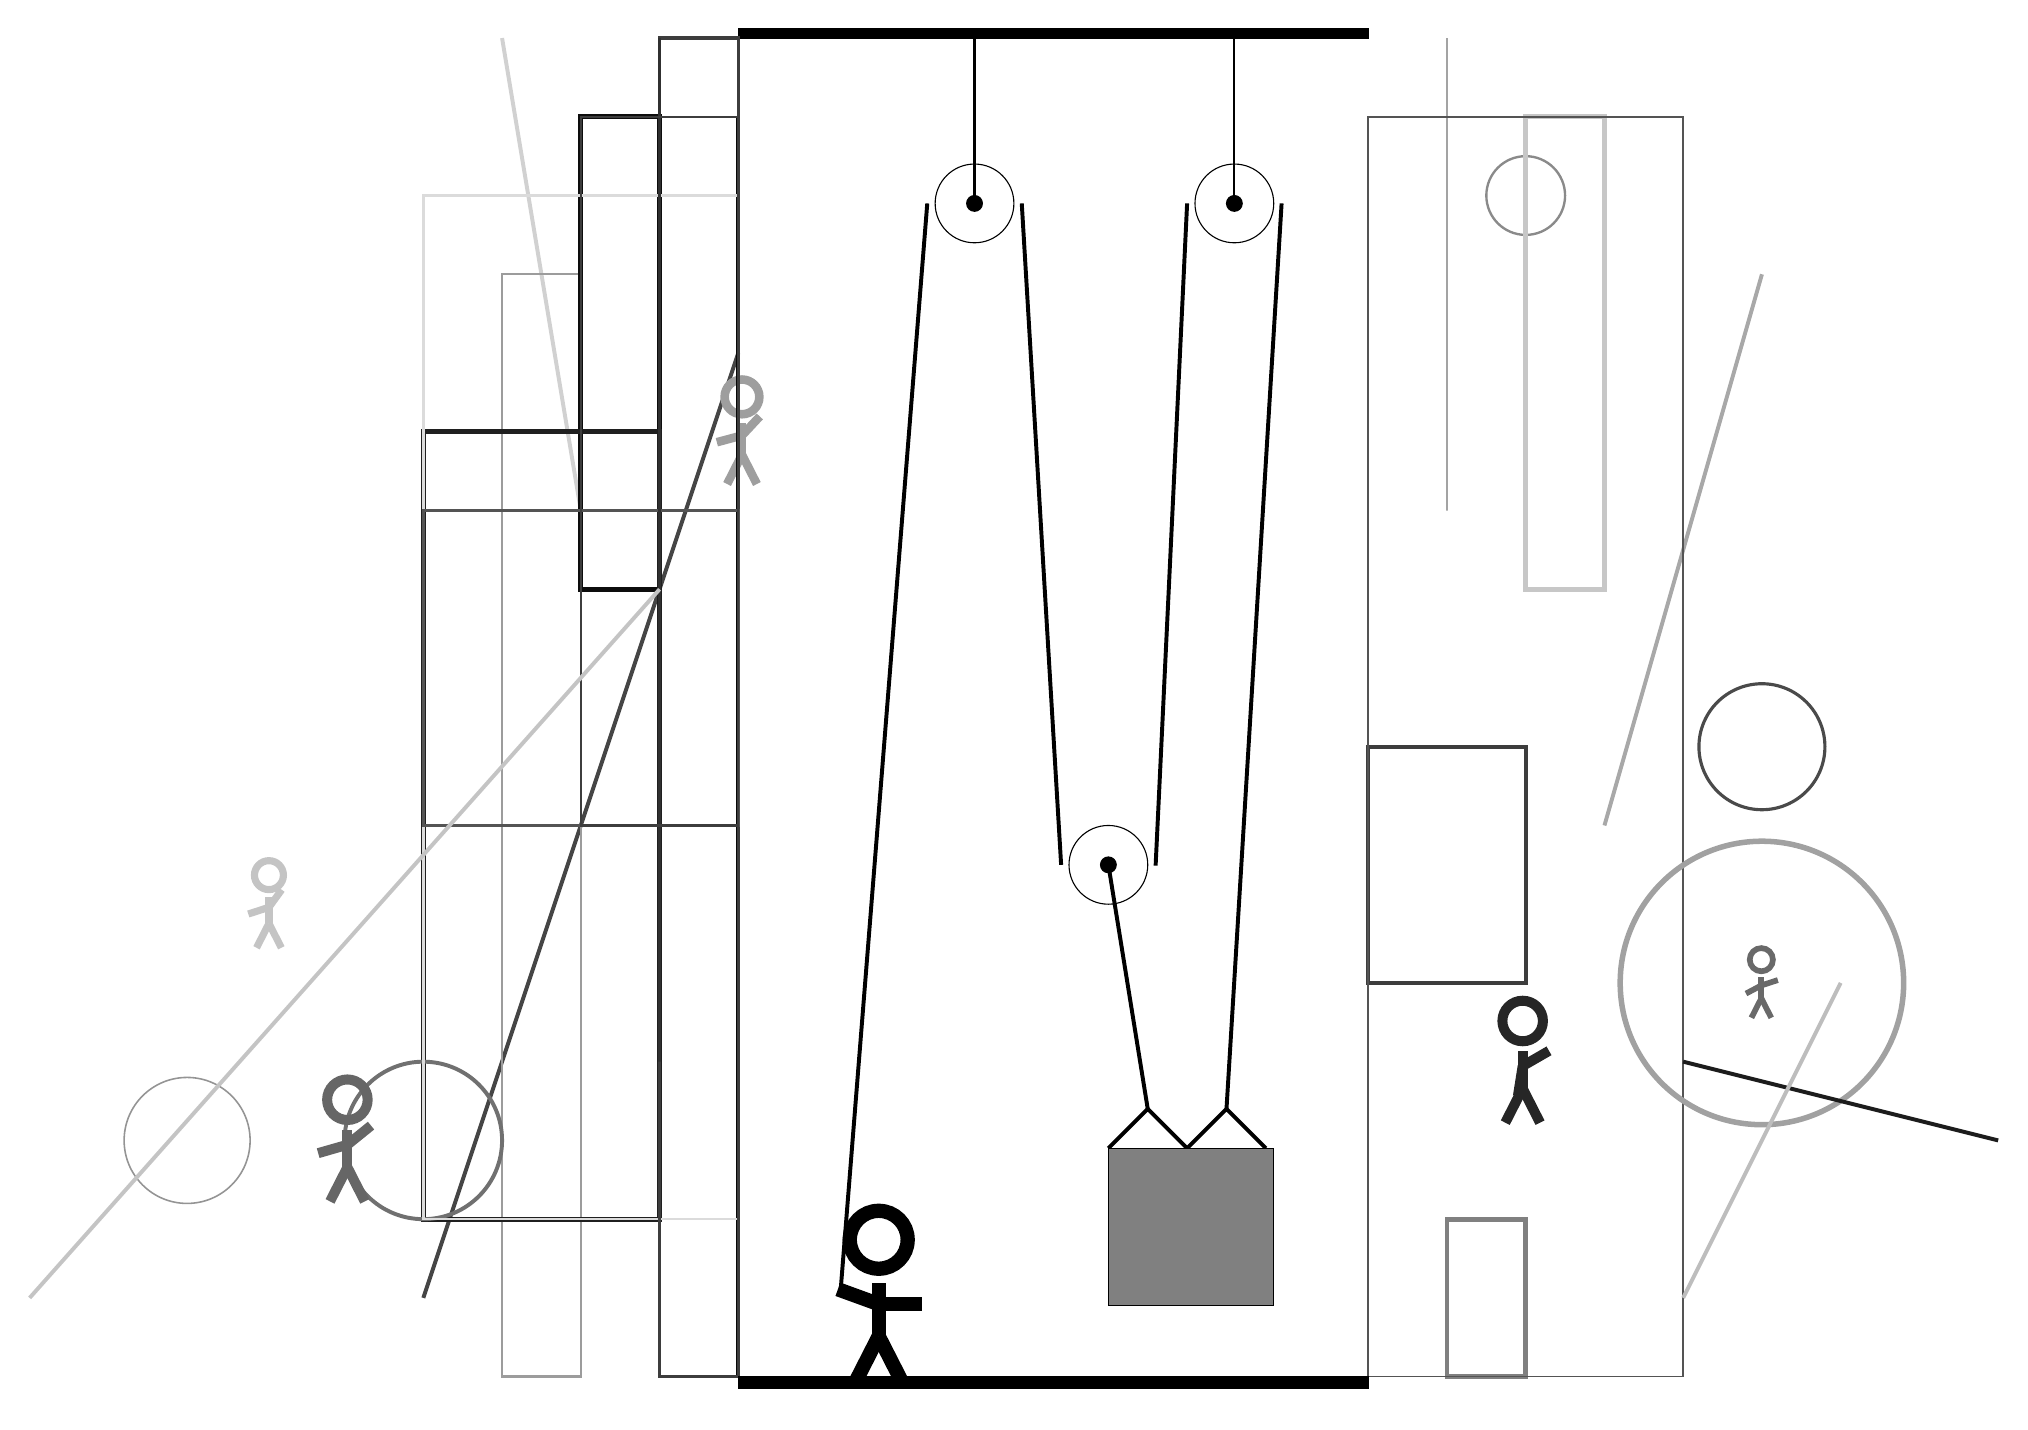
\begin{tikzpicture}
			%%%%% START %%%%%
			
			\draw[fill=black] (-2, 14) rectangle (6, 14.125);
			
			\draw (1, 11.9) circle (0.5);
			\draw[fill=black] (1, 11.9) circle (0.1);
			\draw[thick] (1, 11.9) -- (1, 14);
			
			\draw (4.3, 11.9) circle (0.5);
			\draw[fill=black] (4.3, 11.9) circle (0.1);
			\draw[thick] (4.3, 11.9) -- (4.3, 14);
			
			\draw (2.7, 3.5) circle (0.5);
			\draw[fill=black] (2.7, 3.5) circle (0.1);
			
			\draw[line width=0.5mm]  (2.7, -0.1) -- (3.2, 0.4) -- (3.7, -0.1) -- (4.2, 0.4) -- (4.7, -0.1);
			\draw[fill=black!50] (2.7, -0.1) rectangle (4.8, -2.1);
			
			\draw[line width=0.6mm, color=black!50] (8, -1) rectangle (7, -3);
			
			\draw[line width=0.5mm, color=black!73](-2, 10) -- (-6, -2);
			\draw[line width=0.5mm, color=black!18](-4, 8) -- (-5, 14);
			\draw[line width=0.5mm, color=black!34](9, 4) -- (11, 11);
			\draw[line width=0.3mm, color=black!39] (-4, 11) rectangle (-5, -3);
			\draw[line width=0.2mm, color=black!36] (7, 8) rectangle (7, 14);
			
			\draw[line width=0.6mm, color=black!95] (-3, 7) rectangle (-4, 13);
			\draw[line width=0.5mm, color=black!76] (6, 5) rectangle (8, 2);
			\draw [line width=0.2mm, color=black!42](-9, 0) circle (0.8);
			
			\node[line width=0.4mm, color=black!23] at (-8, 3) {\Strichmaxerl[5][18][54]};
			
			\draw [line width=0.4mm, color=black!71](11, 5) circle (0.8);
			\node[line width=0.5mm, color=black!38] at (-2, 9) {\Strichmaxerl[6][15][47]};
			\draw [line width=0.3mm, color=black!46](8, 12) circle (0.5);
			\draw[line width=0.6mm, color=black!88] (-3, 9) rectangle (-6, -1);
			\draw[line width=0.6mm, color=black!22] (8, 13) rectangle (9, 7);
			\draw [line width=0.5mm, color=black!56](-6, 0) circle (1.0);
			\draw[line width=0.5mm, color=black!97](-2, 13) -- (-2, -3);
			\node[line width=0.7mm, color=black!59] at (11, 2) {\Strichmaxerl[4][28][18]};
			\draw[line width=0.3mm, color=black!14] (-2, -1) rectangle (-6, 12);
			
			\draw[line width=0.4mm, color=black!76] (-2, -3) rectangle (-3, 14);
			\draw[line width=0.2mm, color=black!67] (6, 13) rectangle (10, -3);
			
			\draw[line width=0.4mm, color=black!67] (-2, 4) rectangle (-6, 8);
			\draw[line width=0.3mm, color=black!81] (-3, 1) rectangle (-3, 14);
			\draw [line width=0.7mm, color=black!37](11, 2) circle (1.8);
			\draw[line width=0.3mm, color=black!76] (-4, 4) rectangle (-2, 13);
			
			\node[line width=0.2mm, color=black!85] at (8, 1) {\Strichmaxerl[7][81][30]};
			\draw[line width=0.5mm, color=black!23](-3, 7) -- (-11, -2);
			\draw[line width=0.5mm, color=black!89](10, 1) -- (14, 0);
			\node[line width=0.6mm, color=black!60] at (-7, 0) {\Strichmaxerl[7][16][39]};
			
			\draw[line width=0.5mm, color=black!26](10, -2) -- (12, 2);
			
			\draw[line width=0.5mm](-0.7, -1.9) -- (0.4, 11.9);
			\centerarc[line width=0.5mm](1, 11.9)(0:180:0.6);
			\draw[line width=0.5mm](1.6, 11.9) -- (2.1, 3.5);
			\centerarc[line width=0.5mm](2.7, 3.5)(180:370:0.6);
			\draw[line width=0.5mm] (3.3, 3.49) -- (3.7, 11.9);
			\centerarc[line width=0.5mm](4.3, 11.9)(0:180:0.6);
			\draw[line width=0.5mm](4.2, 0.4) -- (4.9, 11.9);
			\draw[line width=0.5mm] (3.2, 0.4) -- (2.7, 3.5);
			
			\node at (-0.2, -2) {\Strichmaxerl[10][-20][0]};
			
			\draw[fill=black] (-2, -3) rectangle (6, -3.15);
			
			%%%%% END %%%%%
		\end{tikzpicture}
	\end{figure}	
\end{document}